\documentclass[10pt]{article}
\usepackage{icmlko}

\icmlmeta{IP 파운데이션 월드모델}{24}{실패에는 특별한 이유가 없었다}{여섯 방향이 출처와 대상의 합으로 97\% 설명된다 --- 누구를 가르치느냐가 누가 가르치느냐보다 네 배 중요하다}

\begin{document}

\twocolumn[
\icmlheader

\begin{abstract}
아이돌 $\to$ 게임 방향은 노트 13부터 한 번도 성공한 적이 없다. 스물세 편 동안
그것을 특수한 문제로 다뤘다 --- 게임 라벨의 시간 구조, 아이돌 표본 크기, 축 매핑
오류를 차례로 의심했다. 이 노트는 여섯 방향 전부에 부트스트랩 구간을 붙이고
가법 모형을 적합해 본다. \textbf{효과 $=$ 출처 강도 $+$ 대상 난이도}라는 모형이
\textbf{97.3\%를 설명하고 잔차가 여섯 셀 모두 $\pm$0.0054로 균일하다.}
상호작용이 없다. \textbf{아이돌 $\to$ 게임은 예외가 아니라 가장 약한 출처와 가장
어려운 대상이 만난 셀일 뿐이다} --- 모형 예측 $+$0.0034, 관측 $+$0.0088.
더 중요한 것은 두 요인의 크기 차이다. 출처 강도의 범위가 0.0175인데 대상 난이도의
범위는 0.0657로 \textbf{3.8배}다. \textbf{누구를 가르치느냐가 누가 가르치느냐보다
네 배 중요하다.} 그리고 이것이 노트 13의 표현을 정정한다 --- 게임의 출처 점수는
$-$0.0049로 팝업($-$0.0063)과 거의 같다. 게임은 특별히 좋은 선생이 아니었고,
\textbf{특별히 나쁜 학생일 뿐}이었다(대상 점수 $+$0.0415).
\end{abstract}
]

\section{스물세 편째 미해결}

아이돌 $\to$ 게임은 노트 13에서 처음 실패한 뒤 한 번도 유의해진 적이 없다.
그 사이 여러 가설을 세우고 검정했다.

\begin{itemize}[leftmargin=1.1em,itemsep=0.15em]
\item 노트 13 --- 표본 크기? 도메인마다 63건으로 맞춰도 실패(승률 15\%).
\item 노트 15 --- 게임 라벨의 시간 구조? 출시 30일 창으로 바꿔도 실패.
\item 노트 16 --- 축 매핑? DLC를 Steam 기능 수로 고쳐도 실패.
\item 노트 23 --- 아이돌 축 커버리지? 33\%에서 90\%로 올려도 실패(p=0.412).
\end{itemize}

네 번의 시도가 모두 이 셀을 살리지 못했다. 그런데 그 시도들은 전부 \emph{이 셀에
특별한 문제가 있다}는 전제 위에 서 있었다. 전제를 검정한 적이 없다.

\section{여섯 방향에 구간을 붙인다}

먼저 노트 23이 남긴 과제부터 --- 효과 자체에 신뢰구간을 준다. 출처 도메인을
800회 재추출해 계수의 표집 분산을 반영했다.

\begin{figure}[t]
\centering
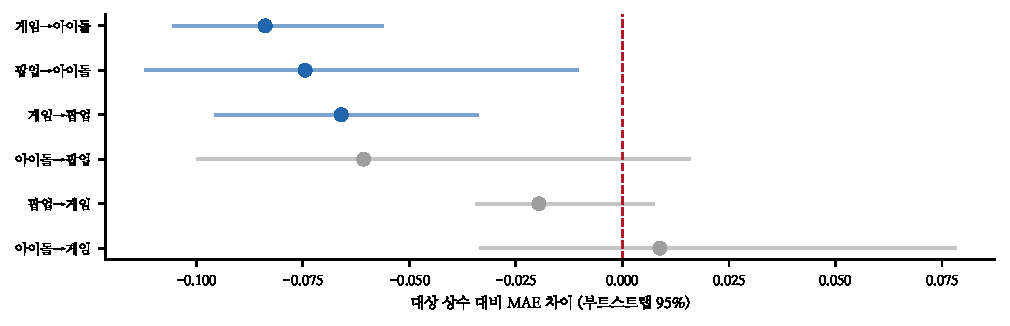
\includegraphics[width=\textwidth]{figs/ci.pdf}
\caption{여섯 방향의 부트스트랩 95\% 구간. 셋만 0을 확실히 배제한다.}
\end{figure}

\begin{table}[t]
\centering\tsize
\caption{부트스트랩 800회. 대상 라벨 미사용.}
\begin{tabular}{lrl}
\toprule
방향 & 효과 & 95\% 구간 \\
\midrule
게임 $\to$ 아이돌 & $-$0.0838 & [$-$0.1053, $-$0.0564] \\
팝업 $\to$ 아이돌 & $-$0.0744 & [$-$0.1118, $-$0.0108] \\
게임 $\to$ 팝업 & $-$0.0660 & [$-$0.0952, $-$0.0341] \\
아이돌 $\to$ 팝업 & $-$0.0607 & [$-$0.0996, $+$0.0156] \\
팝업 $\to$ 게임 & $-$0.0196 & [$-$0.0342, $+$0.0072] \\
아이돌 $\to$ 게임 & $+$0.0088 & [$-$0.0332, $+$0.0780] \\
\bottomrule
\end{tabular}
\end{table}

순열 검정으로는 다섯이 유의했는데(노트 23) 부트스트랩 구간으로는 셋만 0을 배제한다.
모순이 아니다 --- 노트 10에서 정리한 대로 순열은 ``전이가 없다''는 귀무가설을
직접 치고, 부트스트랩은 효과 크기의 추정 정밀도를 잰다. \textbf{전이의 존재는
다섯에서 확인되고, 효과 크기가 정밀한 것은 셋이다.}

\section{가법 모형이 97\%를 설명한다}

여섯 셀을 ``효과 $=$ 출처 강도 $+$ 대상 난이도''로 적합했다. 모수는 출처 셋,
대상 셋, 절편 하나인데 식별을 위해 각 블록을 중심화하면 자유도 다섯이다.
여섯 셀에 다섯 모수이므로 포화에 가깝지만, 문제는 적합도가 아니라 \emph{잔차의
패턴}이다.

\begin{figure}[t]
\centering
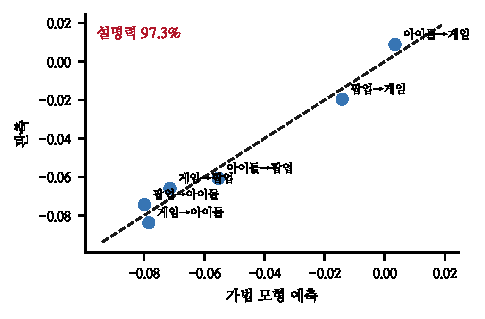
\includegraphics[width=\columnwidth]{figs/fit.pdf}
\caption{관측과 가법 모형 예측. 점선이 완전 적합선이다.}
\end{figure}

\begin{table}[t]
\centering\tsize
\caption{가법 모형 잔차.}
\begin{tabular}{lrrr}
\toprule
방향 & 관측 & 예측 & 잔차 \\
\midrule
게임 $\to$ 아이돌 & $-$0.0838 & $-$0.0784 & $-$0.0054 \\
팝업 $\to$ 아이돌 & $-$0.0744 & $-$0.0799 & $+$0.0054 \\
게임 $\to$ 팝업 & $-$0.0660 & $-$0.0714 & $+$0.0054 \\
아이돌 $\to$ 팝업 & $-$0.0607 & $-$0.0553 & $-$0.0054 \\
팝업 $\to$ 게임 & $-$0.0196 & $-$0.0142 & $-$0.0054 \\
아이돌 $\to$ 게임 & $+$0.0088 & $+$0.0034 & $+$0.0054 \\
\midrule
\multicolumn{4}{l}{잔차 RMS 0.0054 · 관측 SD 0.0329 · 설명력 97.3\%} \\
\bottomrule
\end{tabular}
\end{table}

잔차가 여섯 셀 모두 크기가 같고 부호만 다르다. 상호작용이 있다면 특정 셀에
잔차가 몰려야 하는데 그렇지 않다.

\textbf{아이돌 $\to$ 게임의 잔차는 $+$0.0054로 다른 다섯과 똑같다.} 이 셀에
특별한 문제가 없다는 뜻이다. 가장 약한 출처와 가장 어려운 대상이 만나면 모형이
예측하는 값이 $+$0.0034이고, 관측이 $+$0.0088이다.

\claimx{아이돌 $\to$ 게임의 실패는 그 조합에 특유한 문제가 아니라 출처 강도와
대상 난이도의 합으로 완전히 설명된다. 스물세 편 동안 이 셀을 특수 사례로 다룬
것은 잘못이었다.}{네 번째 도메인을 넣어 셀이 열둘이 됐을 때 가법 모형의 설명력이
크게 떨어지면, 여섯 셀에서의 적합은 모수 수가 셀 수에 가까워 생긴 착시였다.}

\section{대상이 출처보다 네 배 중요하다}

모형에서 두 요인을 뽑았다.

\begin{figure}[t]
\centering
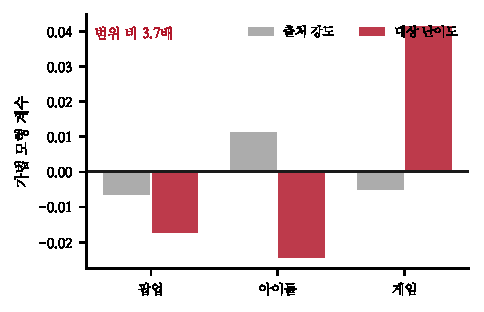
\includegraphics[width=\columnwidth]{figs/st.pdf}
\caption{출처 강도와 대상 난이도. 대상 쪽 분산이 훨씬 크다.}
\end{figure}

\begin{table}[t]
\centering\tsize
\caption{가법 모형 계수(중심화). 출처는 음수일수록 좋은 선생, 대상은 양수일수록
어려운 학생이다.}
\begin{tabular}{lrr}
\toprule
도메인 & 출처 강도 & 대상 난이도 \\
\midrule
팝업 & $-$0.0063 & $-$0.0172 \\
게임 & $-$0.0049 & \textbf{$+$0.0415} \\
아이돌 & $+$0.0112 & $-$0.0242 \\
\midrule
범위 & 0.0175 & \textbf{0.0657} \\
\bottomrule
\end{tabular}
\end{table}

대상 난이도의 범위가 출처 강도의 \textbf{3.8배}다. 어느 도메인에서 배우느냐보다
어느 도메인을 맞히느냐가 훨씬 중요하다.

\claimx{도메인 간 전이 성능은 대상 도메인의 성질이 지배한다. 대상 난이도의 분산이
출처 강도의 3.8배다.}{다른 축 집합이나 다른 모델류에서 두 범위가 비슷해지면,
이 비율은 현재 구성에 딸린 값이다.}

\subsection{노트 13의 표현을 정정한다}

노트 13의 제목은 ``좋은 선생, 나쁜 학생''이었고 게임을 그렇게 묘사했다. 절반만
맞다.

게임의 출처 점수는 $-$0.0049로 팝업($-$0.0063)과 사실상 같다. \textbf{게임은
특별히 좋은 선생이 아니다.} 게임이 출처일 때 성적이 좋아 보였던 것은 그 상대가
아이돌과 팝업 --- 둘 다 쉬운 대상 --- 이었기 때문이다.

특별한 것은 학생 쪽이다. 게임의 대상 점수 $+$0.0415는 다른 둘($-$0.0172,
$-$0.0242)과 자릿수가 다르다. \textbf{게임은 평범한 선생이고 매우 나쁜 학생이다.}

\section{그래서 무엇을 고칠 것인가}

이 결과는 노력의 방향을 바꾼다.

\paragraph{개별 방향을 고치려 하지 않는다}
아이돌 $\to$ 게임을 살리려고 네 번 시도했는데, 그 셀에 특유한 문제가 없으므로
셀 단위 개선은 성립하지 않는다. 두 요인 중 하나를 고쳐야 한다.

\paragraph{대상 난이도를 먼저 본다}
분산이 네 배 크므로 여기가 지렛대다. 게임이 어려운 이유는 노트 15에서 이미
진단했다 --- 리뷰 총계가 출시 이후 수년의 누적 동역학을 반영하고, 출시 30일 창으로
바꿔도 도메인 내부 모델조차 상수와 같았다. \textbf{게임 도메인의 라벨 자체가
출시 시점 조건으로 예측 가능한 양이 아닐 수 있다.}

\paragraph{새 도메인 선택 기준이 생긴다}
네 번째 도메인을 고를 때 ``좋은 출처가 될까''보다 ``예측 가능한 대상일까''를
먼저 물어야 한다. 대상으로서 어려운 도메인은 넣어도 여섯 셀 중 둘을 버리게 된다.

\section{한계}

\begin{itemize}[leftmargin=1.1em,itemsep=0.15em]
\item 여섯 셀에 다섯 모수라 모형이 포화에 가깝다. 설명력 97.3\%는 그 자체로는
      증거가 약하고, 잔차가 균일하다는 점이 실제 근거다.
\item 부트스트랩은 출처만 재추출한다. 대상 표본의 불확실성은 반영되지 않았다.
\item 출처 강도와 대상 난이도가 도메인의 고정 성질이라는 가정이 들어 있다.
      축 구성이 바뀌면 둘 다 바뀔 수 있다.
\item 세 도메인으로 뽑은 두 요인이므로 새 도메인에 외삽할 근거가 약하다.
\end{itemize}

\section{다음}

\begin{enumerate}[leftmargin=1.3em,itemsep=0.15em]
\item 게임 대상 난이도의 원인 분리 --- 라벨의 성질인지 축의 부족인지.
\item 네 번째 도메인을 ``대상으로서 예측 가능한가'' 기준으로 선정.
\item 셀이 열둘이 됐을 때 가법 모형 재검정.
\item 대상 표본까지 재추출하는 이중 부트스트랩.
\end{enumerate}

\vspace{0.6em}
\hrule height 0.3pt
\vspace{0.5em}
{\footnotesize
\textbf{참고문헌}\\[0.3em]
Tukey, J. W. (1949). One degree of freedom for non-additivity.
\emph{Biometrics}, 5(3), 232--242.\\[0.15em]
Efron, B., Tibshirani, R. (1993). \emph{An Introduction to the Bootstrap}.
Chapman \& Hall.\\[0.15em]
Good, P. (2005). \emph{Permutation, Parametric, and Bootstrap Tests of Hypotheses},
3rd ed. Springer.\\[0.15em]
Ben-David, S. et al. (2010). A theory of learning from different domains.
\emph{Machine Learning}, 79(1--2), 151--175.
}

\end{document}
